\section[Local refinement]{Locally refined meshes}

\begin{frame}
  \frametitle{Hanging nodes}
  \begin{center}
    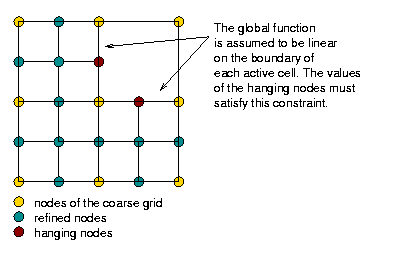
\includegraphics[height=.5\textheight]{graph/hanging_nodes}    
  \end{center}
  \begin{itemize}
  \item Basis functions must be conforming
    \item Constraints on the refined side
    \begin{itemize}
      \item Algebraic
      \item Only depend on shape functions and node functionals
      \item Can be precomputed for every finite element
    \end{itemize}
  \item Constrained degrees of freedom do not actually exist
    \begin{itemize}
    \item Should remain zero during linear solving
    \item Must be set correctly for visualization
    \end{itemize}
  \end{itemize}
\end{frame}

\begin{frame}
  \frametitle{\lstinline!ConstraintMatrix!}
  Constrains hanging nodes and boundary values
  \begin{itemize}
  \item \lstinline!ConstraintMatrix::distribute_local_to_global()!
    \begin{itemize}
    \item Assembles cell matrices and vectors into global vectors
    \item Ensures all constrained degrees of freedom remain zero
    \end{itemize}
  \item \lstinline!ConstraintMatrix::distribute()!
    \begin{itemize}
    \item Modifies a constrained global vector such that the finite
      element function can be evaluated for quadrature and
      visualization
    \end{itemize}
  \end{itemize}
\end{frame}

\begin{frame}
  \frametitle{Adaptive refinement}
  \begin{itemize}
  \item Refinement indicator
    \begin{itemize}
    \item Error estimator
    \item Roughness indicator (Zienkiewicz/Zhou, Kelly et all)
    \end{itemize}
  \item Refinement strategy
    \begin{itemize}
    \item Refine a certain number of the total number of cells
    \item Refine such that accumulated indicator values are a certain
      fraction of the estimate
    \end{itemize}
  \end{itemize}
\end{frame}
\begin{frame}
  \frametitle{Problem: Poisson equation, local refinement II}
  \begin{enumerate}
  \item Add a \lstinline!ConstraintMatrix! to your main class and fill it, using
    \begin{itemize}
    \item \lstinline!DoFTools::make_zero_boundary_constraints()!
    \item \lstinline!DoFTools::make_hanging_node_constraints()!
    \end{itemize}
  \item Integrate the bilinear form into a \lstinline!FullMatrix! on
    each cell.
  \item Distribute the cell matrix and cell vector using the
    \lstinline!ConstraintMatrix!
  \item After solving, use \lstinline!ConstraintMatrix::distribute()!
    to get the vector into a format that can be displayed
  \item Use \lstinline!KellyErrorEstimator! on an L-shaped domain for
    adaptive refinement
  \end{enumerate}
Hint: if you get stuck, read the documentation or step 6.
\end{frame}

\begin{frame}
  \frametitle{Problem: Poisson equation, local refinement}
  \begin{enumerate}
  \item Use one of the locally refined meshes from the first set of
    exercises and verify that the solution becomes bad
  \item Add a \lstinline!ConstraintMatrix! to your main class and fill it, using
    \begin{itemize}
    \item \lstinline!DoFTools::make_zero_boundary_constraints()!
    \item \lstinline!DoFTools::make_hanging_node_constraints()!
    \end{itemize}
  \item Integrate the bilinear form into a \lstinline!FullMatrix! on
    each cell.
  \item Distribute the cell matrix and cell vector using the
    \lstinline!ConstraintMatrix!
  \item After solving, use \lstinline!ConstraintMatrix::distribute()!
    to get the vector into a format that can be displayed
  \item Use \lstinline!KellyErrorEstimator! on an L-shaped domain for
    adaptive refinement
  \end{enumerate}
Hint: if you get stuck, read the documentation or step 6.
\end{frame}


%%% Local Variables: 
%%% mode: latex
%%% TeX-master: "slides"
%%% End: 
